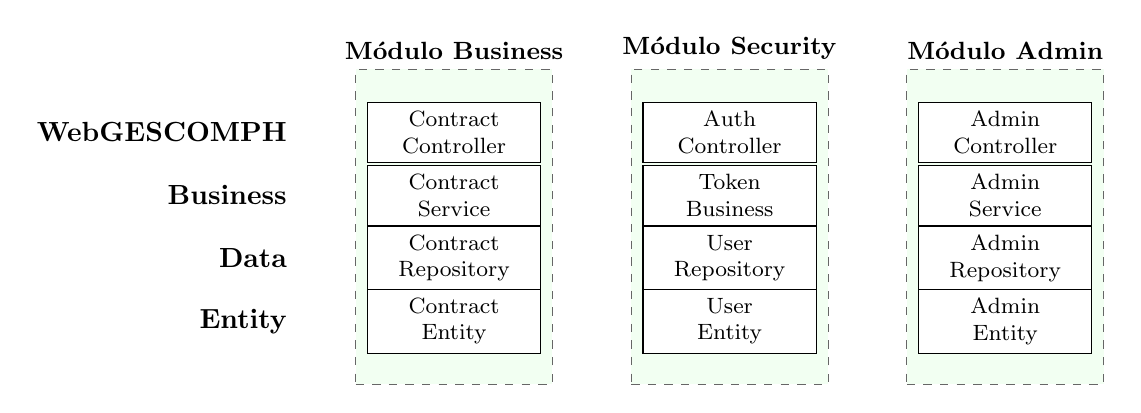
\begin{tikzpicture}[
    every node/.append style={font=\small},
    module/.style={rectangle, draw=black!60, dashed, fill=green!5, minimum width=2.5cm, minimum height=4cm, label=above:\textbf{#1}},
    layer/.style={rectangle, draw=black, fill=white, minimum width=2.2cm, minimum height=0.6cm, align=center, font=\footnotesize}
]
    % Módulo Business
    \node[module=Módulo Business] (modBusiness) at (0,0) {};
    \node[layer] at (0, 1.2) {Contract\\Controller};
    \node[layer] at (0, 0.4) {Contract\\Service};
    \node[layer] at (0, -0.4) {Contract\\Repository};
    \node[layer] at (0, -1.2) {Contract\\Entity};

    % Módulo Security
    \node[module=Módulo Security] (modSecurity) at (3.5,0) {};
    \node[layer] at (3.5, 1.2) {Auth\\Controller};
    \node[layer] at (3.5, 0.4) {Token\\Business};
    \node[layer] at (3.5, -0.4) {User\\Repository};
    \node[layer] at (3.5, -1.2) {User\\Entity};

    % Módulo Admin
    \node[module=Módulo Admin] (modAdmin) at (7,0) {};
    \node[layer] at (7, 1.2) {Admin\\Controller};
    \node[layer] at (7, 0.4) {Admin\\Service};
    \node[layer] at (7, -0.4) {Admin\\Repository};
    \node[layer] at (7, -1.2) {Admin\\Entity};

    % Etiquetas de capas laterales
    \node[anchor=east, font=\bfseries] at (-2, 1.2) {WebGESCOMPH};
    \node[anchor=east, font=\bfseries] at (-2, 0.4) {Business};
    \node[anchor=east, font=\bfseries] at (-2, -0.4) {Data};
    \node[anchor=east, font=\bfseries] at (-2, -1.2) {Entity};

\end{tikzpicture}
